%%%%%%%%%%%%%%%%%%%%%%%%%%%%%%%%%%%%%%%%%%%%%%%%%%%%%%%%%%%%%%%%%%%%%%%%%%%%%%

\documentclass{l3deliverable}

%%%%%%%%%%%%%%%%%%%%%%%%%%%%%%%%%%%%%%%%%%%%%%%%%%%%%%%%%%%%%%%%%%%%%%%%%%%%%%


%%%%%%%%%%%%%%%%%%%%%%%%%%%%%%%%%%%%%%%%%%%%%%%%%%%%%%%%%%%%%%%%%%%%%%%%%%%%%%
% a utility environment for formatting tasks - see document for usage
\usepackage{tabulary}
\newenvironment{PSDTask}[2]{
  \tabularx{\linewidth}{|l|X|} \hline
    \bf\itshape Task #1: & \bf\itshape #2 \\\hline
}{\endtabularx}

\newcommand{\PSDTaskComponent}[2]{\it #1: & #2 \\ \hline}
\newcommand{\PSDTaskDescription}[1]{\PSDTaskComponent{Description}{#1}}
\newcommand{\PSDTaskOutcomes}[1]{\PSDTaskComponent{Outcomes}{#1}}
\newcommand{\PSDTaskDeliverables}[1]{\PSDTaskComponent{Deliverables}{#1}}
\newcommand{\PSDTaskRisks}[1]{\PSDTaskComponent{Risk}{#1}}

%%%%%%%%%%%%%%%%%%%%%%%%%%%%%%%%%%%%%%%%%%%%%%%%%%%%%%%%%%%%%%%%%%%%%%%%%%%%%%

\usepackage{url}

%%%%%%%%%%%%%%%%%%%%%%%%%%%%%%%%%%%%%%%%%%%%%%%%%%%%%%%%%%%%%%%%%%%%%%%%%%%%%%
%% Check these macro values for appropriateness for your own document.

\title{Project Plan}

%%authors
\author{
  Ross Adam \\
  Andrew Gardner \\
  Nicole Kearns \\
  Mamas Nicolau \\
  Asset Sarsengaliyev \\
  ...}

%%release date
\date{10 January 2009}

\deliverableID{D2}
\project{PSD Group Exercise 1}
\team{X}

%%%%%%%%%%%%%%%%%%%%%%%%%%%%%%%%%%%%%%%%%%%%%%%%%%%%%%%%%%%%%%%%%%%%%%%%%%%%%%

\begin{document}

%%%%%%%%%%%%%%%%%%%%%%%%%%%%%%%%%%%%%%%%%%%%%%%%%%%%%%%%%%%%%%%%%%%%%%%%%%%%%%

\maketitle

\tableofcontents

\newpage

%%%%%%%%%%%%%%%%%%%%%%%%%%%%%%%%%%%%%%%%%%%%%%%%%%%%%%%%%%%%%%%%%%%%%%%%%%%%%%
%% Standard section for all documents

\section{Introduction}

\subsection{Identification}

Project plan for the internship system for PSD3 team project.

\subsection{Related Documentation}

{{PSD3 Group Exercise Description \url{http://fims.moodle.gla.ac.uk/file.php/128/coursework/psd3-ge-1-rev3278.pdf}}\\

Deliverables Template \url{http://fims.moodle.gla.ac.uk/file.php/128/coursework/templates.zip}\\

PSD3 Course Notes \url{http://fims.moodle.gla.ac.uk/file.php/128/lecture-notes/notes-r3275.pdf}\\

\subsection{Purpose and Description of Document}

The purpose of this document is to detail and explain the tasks which will be involved in the development of the intenship sytem and to identify and explain any risks which may be involved.

\subsection{Document Status and Schedule}

\begin{center}{
\begin{tabular}{|c|c|c|c|}
\hline \textbf{Date} &\textbf{Change} & \textbf{Version} & \textbf{Author}\\ 
\hline 02/10/2012 & Began Draft & 0.1 & All \\ 
\hline 09/10/2012 & Initial Draft Completed & 0.2 & All \\ 
\hline 10/10/2012 & Finalised for Submission & 0.3 & All\\ 
\hline 11/10/2012 & \textbf{Draft Submission Deadline} & 1.0 & All\\ 
\hline
\hline 26/11/2012 & Completed introduction section & 1.1 & All\\
\hline 26/11/2012 & Modified and Added Tasks & 1.2 & All\\ 
\hline & \textbf{ADD MORE HERE!} & & All\\
\hline  & Finalised for Submission &  & All\\
\hline 29/11/2012 & \textbf{Final Submission Deadline} &  & \\ 
\hline 
\end{tabular} }
\end{center}

%%%%%%%%%%%%%%%%%%%%%%%%%%%%%%%%%%%%%%%%%%%%%%%%%%%%%%%%%%%%%%%%%%%%%%%%%%%%%%

\section{Resources, Budgets, Schedules and Organisation}

%%%%%%%%%%%%%%%%%%%%%%%%%%%%%%%%%%%%%%%%%%%%%%%%%%%%%%%%%%%%%%%%%%%%%%%%%%%%%%

\subsection{Work Breakdown Structure}

Describe the logical structure for managing acquisition and
development (or relevant subsection thereof) by means of a Work
Breakdown Structure (WBS) scheme that is coordinated with the resource
allocation described in Subsection \ref{sec:allocation}. An
activities-oriented rather than an organisation- or product oriented
WBS is recommended. The level of detail given in the WBS should be
sufficient to support sound management practices.

For purposes of the WBS, identify the activities to be
undertaken. Define these in terms of a descriptive statement in
operational terms of activities and identification of the products to
be delivered or outcomes of the activity.

For each activity give: 

\begin{itemize}
\item an identifying label;
\item a descriptive statement in operational terms (what needs to be
  done);
\item identification of outcomes, including deliverables; and
\item a brief risk assessment.
\end{itemize}

For example, using the PSDTask environment (defined in this document's
header):

\begin{PSDTask}{1}{Breakdown of Initial Problem Definition}
  \PSDTaskDescription{ Discussing the initial problems and forming our own ideas of how to approach the client's task.}%
  \PSDTaskOutcomes{Problem breakdown.}%
  \PSDTaskDeliverables{None}%
  \PSDTaskRisks{R1}
\end{PSDTask}

\begin{PSDTask}{2}{Identify Initial Requirements}
  \PSDTaskDescription{ Using the initial problem definition, identify what the basic features of the system should be.}%
  \PSDTaskOutcomes{Inital requirements list}%
  \PSDTaskDeliverables{None}%
  \PSDTaskRisks{R1}
\end{PSDTask}

\begin{PSDTask}{3}{Prepare Interview Plan}
  \PSDTaskDescription{ Construct questions for Customer Liaison to ask the client in order to elicit requirements. Questions will then be approved by group. An interview plan will then be written consisting of these questions.}%
  \PSDTaskOutcomes{Interview Plan document.}%
  \PSDTaskDeliverables{None}%
  \PSDTaskRisks{R2}
\end{PSDTask}

\begin{PSDTask}{4}{Conduct Interview}
  \PSDTaskDescription{ Meeting with client to collect requirements using the Interview Plan document. If additional information is revealed plan document will be deviated from.}%
  \PSDTaskOutcomes{Interview notes - system requirements}%
  \PSDTaskDeliverables{None}%
  \PSDTaskRisks{R3}
\end{PSDTask}

\begin{PSDTask}{5}{Review Interview Notes}
  \PSDTaskDescription{Look over the notes gathered in the interview with the client and the initial requirements.}%
  \PSDTaskOutcomes{None}%
  \PSDTaskDeliverables{None}%
  \PSDTaskRisks{R1, R3}
\end{PSDTask}

\begin{PSDTask}{6}{Produce Requirements Post Interview}
  \PSDTaskDescription{Produce a document containing all requirements gathered for the system from the client interview.}%
  \PSDTaskOutcomes{Requirements document}%
  \PSDTaskDeliverables{None}%
  \PSDTaskRisks{R1, R3}
\end{PSDTask}

\begin{PSDTask}{7}{Review Initial Requirements}
  \PSDTaskDescription{Check over the requirements document to ensure it contains all requirements for the system, and that they are appropriate for the system}%
  \PSDTaskOutcomes{}%
  \PSDTaskDeliverables{None}%
  \PSDTaskRisks{}
\end{PSDTask}

\begin{PSDTask}{8}{Create UML of Internship Management System}
  \PSDTaskDescription{Produce a UML diagram of the system to show the structure of the internship system}%
  \PSDTaskOutcomes{UML diagram}%
  \PSDTaskDeliverables{D3}%
  \PSDTaskRisks{R6}
\end{PSDTask}

\begin{PSDTask}{9}{Create Use Cases}
  \PSDTaskDescription{ For each of the requirements gathered, produce a use case containing all appropriate information ie. description, actors, conditions,etc}%
  \PSDTaskOutcomes{Requirements Specification}%
  \PSDTaskDeliverables{D3}%
  \PSDTaskRisks{R1}
\end{PSDTask}

\begin{PSDTask}{10}{Create Use Case Diagrams}
  \PSDTaskDescription{ Produce use case diagrams to show the relationship between different use cases and the actors involved.}%
  \PSDTaskOutcomes{Requirements Specification}%
  \PSDTaskDeliverables{D3}%
  \PSDTaskRisks{R1, R6}
\end{PSDTask}

\begin{PSDTask}{11}{Prepare Stakeholders Panel Interview Questions}
  \PSDTaskDescription{Come up with a few key questions about the system/requirements we are unsure about to ask the clients. Allows us to clarify the requirements we have are correct.}%
  \PSDTaskOutcomes{Stakeholder panel Questions}%
  \PSDTaskDeliverables{None}%
  \PSDTaskRisks{R2}
\end{PSDTask}

\begin{PSDTask}{12}{Attend Stakeholders Panel Interview}
  \PSDTaskDescription{Allow the teams to ask questions about the system that maybe were not clear in the interview; or ask questions which they forgot about during the interview.}%
  \PSDTaskOutcomes{Stakeholder panel notes}%
  \PSDTaskDeliverables{None}%
  \PSDTaskRisks{R3}
\end{PSDTask}

\begin{PSDTask}{13}{Review Notes from Stakeholders Panel Interview}
  \PSDTaskDescription{Go through the notes from the stakeholder panel and amend the requirements document where necessary.}%
  \PSDTaskOutcomes{}%
  \PSDTaskDeliverables{None}%
  \PSDTaskRisks{R1, R3}
\end{PSDTask}

\begin{PSDTask}{14}{Finalise all Requirements}
  \PSDTaskDescription{Gather all requirements from the interview and the stakeholder panel and ensure that all the requirements are included in the document}%
  \PSDTaskOutcomes{Final Requirements Document}%
  \PSDTaskDeliverables{}%
  \PSDTaskRisks{}
\end{PSDTask}

\begin{PSDTask}{15}{Finalised UML of Internship Management System}
  \PSDTaskDescription{Modified the UML diagram to suit the requirements gathered at the stakeholder panel}%
  \PSDTaskOutcomes{UML diagram}%
  \PSDTaskDeliverables{D3}%
  \PSDTaskRisks{}
\end{PSDTask}

\begin{PSDTask}{16}{Finalised Use Cases}
  \PSDTaskDescription{Modified the use cases to suit the requirements gathered at the stakeholder panel}%
  \PSDTaskOutcomes{Requirements Specification}%
  \PSDTaskDeliverables{D3}%
  \PSDTaskRisks{}
\end{PSDTask}


\begin{PSDTask}{17}{Finalised Use Case Diagrams}
  \PSDTaskDescription{Modified the use case diagrams to suit the requirements gathered at the stakeholder panel}%
  \PSDTaskOutcomes{Requirements Specification}%
  \PSDTaskDeliverables{D3}%
  \PSDTaskRisks{}
\end{PSDTask}

\begin{PSDTask}{18}{Finalise Requirements Specifications Documents}
  \PSDTaskDescription{Check over the requirements specification to ensure it is correct and contains all relevant information for the use cases, and that the use case diagrams match the information in the descriptions.}%
  \PSDTaskOutcomes{Requirments Specificaiton}%
  \PSDTaskDeliverables{D3}%
  \PSDTaskRisks{}
\end{PSDTask}

\begin{PSDTask}{19}{Research Bash Scripting}
  \PSDTaskDescription{Learn how to do bash scripting in order to create a prototype to show the client the basic functionality of the system and the workflow.}%
  \PSDTaskOutcomes{None}%
  \PSDTaskDeliverables{None}%
  \PSDTaskRisks{}
\end{PSDTask}

\begin{PSDTask}{20}{Create Bash Prototype}
  \PSDTaskDescription{Creating the first actual prototype of the application written in Bash Scripting Language.}%
  \PSDTaskOutcomes{Bash Prototype created}%
  \PSDTaskDeliverables{D4}%
  \PSDTaskRisks{R8}
\end{PSDTask}

\begin{PSDTask}{21}{Test Bash Prototype}
  \PSDTaskDescription{Allow someone to test the prototype created in order to ensure there are no bugs and works as expected.}%
  \PSDTaskOutcomes{}%
  \PSDTaskDeliverables{D4}%
  \PSDTaskRisks{}
\end{PSDTask}

\begin{PSDTask}{22}{Demonstrate Bash Prototype to Customer}
  \PSDTaskDescription{Giving the Customer a first view of how the application functions. The customer will have the opportunity to ask questions and the customer liaison will be available to give answers}%
  \PSDTaskOutcomes{Bash Prototype demonstrated to Customer}%
  \PSDTaskDeliverables{D4}%
  \PSDTaskRisks{}
\end{PSDTask}

\begin{PSDTask}{23}{Review Notes from customer about Bash Prototype}
  \PSDTaskDescription{}%
  \PSDTaskOutcomes{}%
  \PSDTaskDeliverables{D4}%
  \PSDTaskRisks{}
\end{PSDTask}


%%%%%%%%%%%%%%%%%%%%%%%%%%%%%%%%%%%%%%%%%%%%%%%%%%%%%%%%%%%%%%%%%%%%%%%%%%%%%%

\subsection{Resource Estimation and Allocation to WBS\label{sec:allocation}}
The available human resourses for this project are 5 developers as defined in document D1.\\
According to the tasks list (section 2.3) the total estimated duration of this WBS will be 44 hours or 6 working days.\\
\\

Resources Available:\\
Andrew Gardner: Chief Architect \\
Asset Sarsengaliyev: Source Code Manager\\ 
Mamas Nicolaou: Quality Assuror \\
Nicole Kearns: Quality Assuror \\
Ross Adam: Project Manager \\
\\

Resource allocation details are shown in the Task Table below. 

%%%%%%%%%%%%%%%%%%%%%%%%%%%%%%%%%%%%%%%%%%%%%%%%%%%%%%%%%%%%%%%%%%%%%%%%%%%%%%

\subsection{Schedules}

\begin{table}
\caption{Tasks Table} % title of Table
\begin{tabular}{|c |c |c |c |c |} % centered columns (4 columns)
\hline\hline                        %inserts double horizontal lines
Task & Title & Hours & Depend & Team Members \\ [0.5ex]
\hline1 & Breakdown of Initial Problem Definition & 5:00 &-& All\\ % inserting body of the table
\hline3 & &  & & Ross Adam, \\
 &  Prepare Interview Plan&3:00 &2 &Nicole Kearns, \\
 & & & &Asset Sarsengaliyev \\
\hline4 & Conduct Interview & 0:15 &3& All\\
\hline5 & Review Interview Notes& 1:00 &4& All\\
\hline6 & Produce Requirements Post Interview & 1:00 &5& All\\
\hline7 & Review Initial Requirements & 1:00 &6& All \\
\hline8 & Create UML of Internship Management System & 3:00 &7 &Asset Sarsengaliyev, \\
&Internship Management System& & &Nicole Kearns,  \\
& & & & Andrew Gardner \\
\hline9  & Create Use Cases & 2:00&7 &Nicole Kearns,\\
 & & & & Ross Adam \\
\hline10  & Create Use Case Diagrams &2:00 &9 &  Andrew Gardner, \\
 & & & & Mamas Nicolaou \\
\hline11 & Prepare Stakeholders Panel Interview Questions & 1:00 &7& All\\
\hline12 & Attend Stakeholders Panel Interview & 1:00 &11& All\\
\hline13 & Review Notes from Stakeholders Panel Interview & 1:00 &12& All\\
\hline14 & Finalise all Requirements & 2:00 &13& All\\
\hline15 & Finalise UML Diagram of Internship Management System & 1:00 &14& All\\
\hline16 & &  & & Andrew Gardner, \\
 & & & & Mamas Nicolaou, \\
 & Finalise Use Cases & 1:00& 14& \\
\hline17 &  & & & Nicole Kearns, \\
 & & & & Ross Adam, \\
 & Finalise Use Case Diagrams &1:00  &16 & \\
\hline18 & Finalise Requirements Specifications Documents & 2:00 &15,17& Ross Adam \\
\hline19 & Research Bash Scripting & 3:00 &-&Andrew Gardner\\
\hline20 & Create Bash Prototype & 6:00 &19,18&Andrew Gardner \\
\hline21 & Test Bash Prototype & 2:00 &20& Mamas Nicolaou \\
\hline22 & Demonstrate Bash Prototype to Customer & 0.30 &21& All\\     
\hline23 & Review Notes from customer about Bash Prototype & 1:00 &22& All\\      
\hline %inserts single line
\end{tabular}
\label{table:nonlin} % is used to refer this table in the text
\end{table}
\pagebreak

\subsection{Pert Chart}
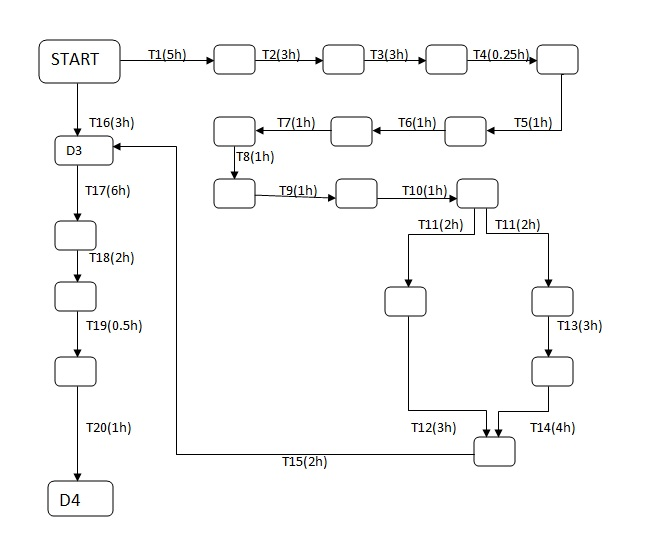
\includegraphics[scale=0.7]{img/PERT.jpg}

\subsection{Gantt Chart}
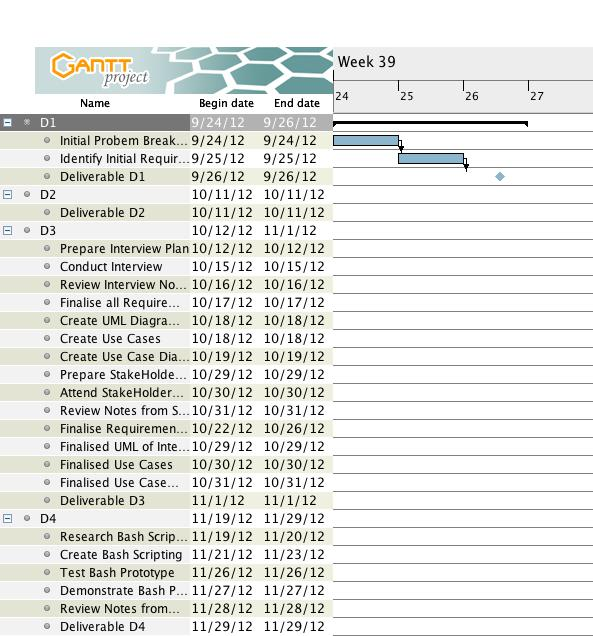
\includegraphics[scale=0.7]{img/GANTT D1.jpg}\\

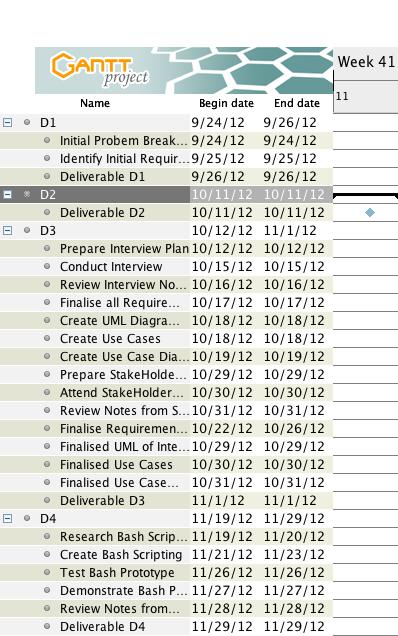
\includegraphics[scale=0.7]{img/GANTT D2.jpg}\\
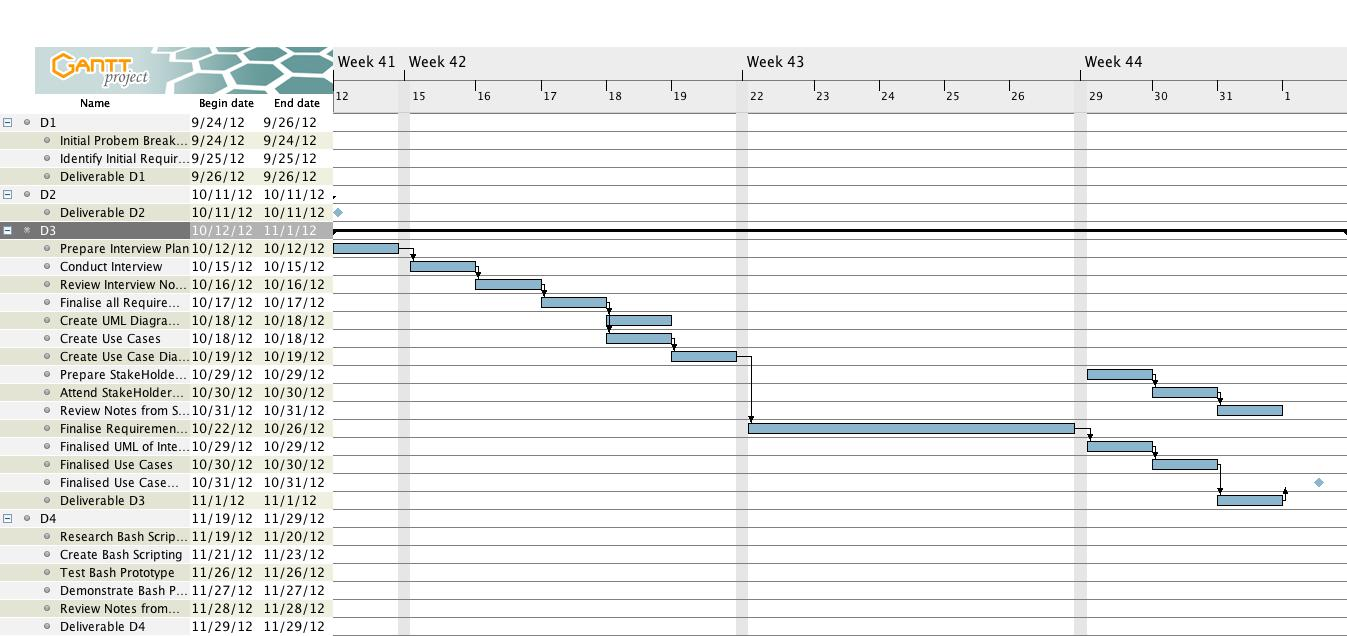
\includegraphics[scale=0.3]{img/GANTT D3.jpg}\\
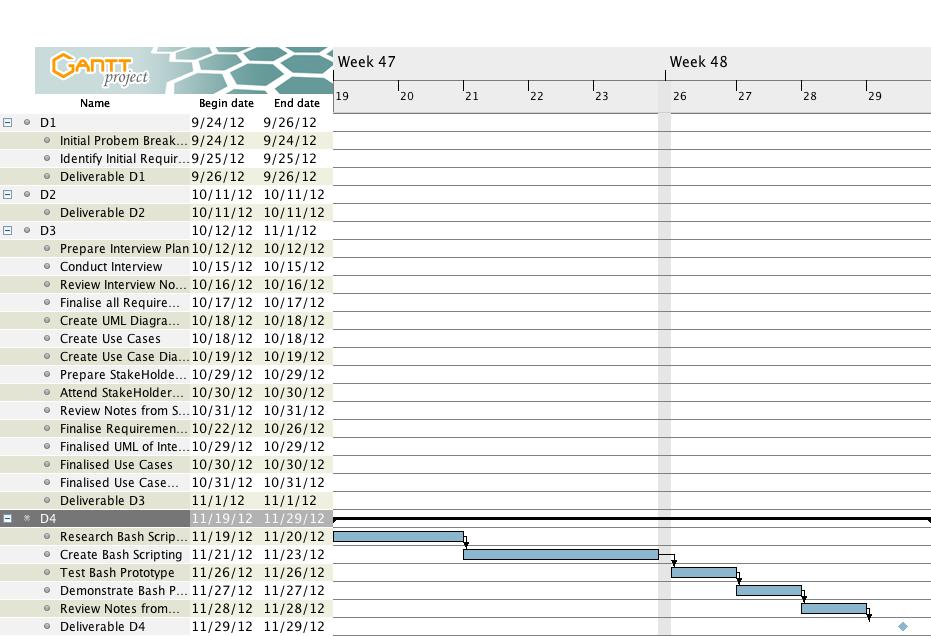
\includegraphics[scale=0.5]{img/GANTT D4.jpg}\\



%%%%%%%%%%%%%%%%%%%%%%%%%%%%%%%%%%%%%%%%%%%%%%%%%%%%%%%%%%%%%%%%%%%%%%%%%%%%%%

\subsection{Equipment, Materials, Facilities, and Other Resources}

%%%%%%%%%%%%%%%%%%%%%%%%%%%%%%%%%%%%%%%%%%%%%%%%%%%%%%%%%%%%%%%%%%%%%%%%%%%%%%

\section{Assurance Plan}


The Quality Assurance Plan(The QAP) is the basis for maintaining the quality of our product on the highest level that matches the requirements for the given software system and approved by stakeholders. The QAP will be overseen by the team to maintain quality improvement activities, such as monitoring, adding features and evaluating defects. The purpose of the QAP is designed to match the following requirements:\\

\begin{itemize}
\item to perform suitable actions when possibilities for improvements in service are identified.\\
\item to implement corrective action when technical issues or bugs are found.\\
\item to ensure that the software system is maintaining properly all the time.\\
\end{itemize}

Our team will mainly rely on Risk Management Plan, Product Requirements Specification and Change Management Plan to keep the product quality to the appropriate level.\\

Team activities:\\

Team members use the special group on Facebook to discuss their thoughts. All the documentation and code are  accessible on GitHub for all members as well as supervisors. It is the responsibility of everyone to ensure that update will not harm any working parts of the system. After altering any part of the code, we invoke test sets to check if the corresponding oracles match expected outputs.\\ 

Team should have one or more meetings every week to discuss the progress of the work. The tasks should be equally divided by team members and this is being added to the timeline of tasks. Every member is in charge of reviewing all finished tasks and task is approved by team if two or more member of the team approves it. \\

Product documentation(Deliverables) are ready to submit when members have no offers how to improve the document. Latex tool is used to produce the documentation.  Feedback for the deliverables is carefully analysed and corrections are done by the whole team at the end of term.\\

In order to make sure the quality of the product will be high and the team is in the right direction, team meets the supervisor every week as well as the clients few times per term.\\

Apart from that, we use black box testing with other teams to check if they can find bugs in prototype, as they have a fresh look to the product.\\

%%%%%%%%%%%%%%%%%%%%%%%%%%%%%%%%%%%%%%%%%%%%%%%%%%%%%%%%%%%%%%%%%%%%%%%%%%%%%%

\section{Risk Management Plan}

\begin{center}{
\begin{tabular}{|p{2cm}|p{2cm}|p{3cm}|p{2cm}|p{3cm}|p{2cm}|}
\hline \textbf{Risk ID} &\textbf{Category} & \textbf{Description} & \textbf{Probability} & \textbf{Impact} & \textbf{Controls}\\
\hline R1 & Requirements & Functional and non-functional requirements may be interpreted differently by team members due to the lack of interviews & Meduim & High / The final product may behave differently and delayed to fix the problems & C1, C3, C5\\
\hline R2 & Requirements & Team members may ask inappropriate questions or miss important requirements & Low & Medium/ This may lead to improper documentation of the product & C2, C8\\
\hline R3 & Requirements & The stakeholders are not sure how the final product should look like & High & Medium/ Stakeholders may not be satisfied with what developers will offer & C1, C3, C5\\
\hline R4 & Skills & Members may over estimate their expectations about the final product & Very high & Medium/ The product will be different from what was offered on documentation & C1, C3, C5\\
\hline R5 & Requirements & Releasing unprofessional document to the client missing some requirements or poorly prepared & Medium & High/ Consequently, the product may not reach expectations & C3, C5, C7\\
\hline R6 & Technical & Team members are unfamiliar with appropriate tools & Medium & High/ Consequently, the product may not reach expectations & C3, C7\\
\hline R7 & Requirements & Tasks may be left from the time-line & Medium & Medium/ This may lead to potential delays & C6\\
\hline R8 & Prototyping & Prototype is not compatible with client's specification & Medium & High/ Changing all specification and possibly start all the work again & C3, C7\\
\hline
\end{tabular} }
\end{center}

\begin{center}{
\begin{tabular}{|c|c|}
\hline \textbf{Control ID} & \textbf{Description}\\
\hline C1 &  Iteratively checking the specification of the product with stakeholders\\
\hline C2 & Prepare the questions with team for the interview\\
\hline C3 & Use other expert advise about the product development\\
\hline C4 & Make presentation of the software system to the stakeholders\\
\hline C5 & Develop the prototype of the product, based on bash script\\
\hline C6 & Check the work by two members of the team\\
\hline C7 & Investigate software competency and other skills within team\\
\hline C8 & Assign one member to conduct the interviews\\
\hline
\end{tabular} }
\end{center}

%%%%%%%%%%%%%%%%%%%%%%%%%%%%%%%%%%%%%%%%%%%%%%%%%%%%%%%%%%%%%%%%%%%%%%%%%%%%%%

\section{Configuration Management Plan}




Describe the activities and plans for configuration management to be
performed by the organization preparing this Management Plan. The
primary topics for the plan include:

\begin{enumerate}
\item Configuration management process
\item Configuration control activities
\item Configuration identification
\item Configuration change control
\end{enumerate}

The contents of this subsection will be explained later in the 1st
semester in the PSD lectures. For initial hand-in deadline, you may
leave this subsection blank or make your best effort to produce an
assurance plan.

%%%%%%%%%%%%%%%%%%%%%%%%%%%%%%%%%%%%%%%%%%%%%%%%%%%%%%%%%%%%%%%%%%%%%%%%%%%%%%

\appendix

\section{Glossary}

\textbf{PSD3:} Professional Software Development 3\\
\textbf{CC:} Course Coordinator\\

\end{document}

%%%%%%%%%%%%%%%%%%%%%%%%%%%%%%%%%%%%%%%%%%%%%%%%%%%%%%%%%%%%%%%%%%%%%%%%%%%%%%

